\section{Contribution}
\subsection{The vertex enumeration for unbounded polyhedra}
\begin{frame}{Changing coordinates}
Requirement: put $0$ in the feasible area and ensure the variables are positive.

\vspace*{0.5cm}

\begin{block}{Finding a vertex}
\begin{itemize}
\item Reach the feasible area (simplex).
\item Pivot the dictionary into obtaining a cobasis constituted only by slack variables.
\item Push the cobasis to its bounds gives a vertex.
\end{itemize}
\end{block}

\end{frame}

\begin{frame}{Detecting the linealty space}

The linealty space is the biggest affine subspace included in the polyhedron.

\vspace*{0.2cm}

\begin{columns}[c]
\begin{column}{5cm}
Example with $-1\leq x+y\leq 1$.\\

\begin{tabular}{| c | c || c c |}
	\hline	
	$x$ & $y$ & & \\
	\hline
	\hline	
   	$-1$ & $-1$ & = & $s_1$\\ \hline	
   	$-1$ & $-1$ & = & $s_2$\\ \hline 
\end{tabular}

\vspace*{0.2cm}

\only<2,3>{\begin{tabular}{| c | c || c c |}
	\hline	
	$s_1$ & $y$ & & \\
	\hline
	\hline	
   	$-1$ & $-1$ & = & $x$\\ \hline	
   	$1$ & $0$ & = & $s_2$\\ \hline 
\end{tabular}

\vspace*{0.2cm}
$(-1,1)$ is a linealty direction.}
\end{column}
\begin{column}{5cm}
\begin{figure}
\only<1,2>{
\includegraphics[scale=1.5]{images/linealty.eps}}
\only<3>{
\includegraphics[scale=1.5]{images/linealty2.eps}}
\end{figure}
\end{column}
\end{columns}


\end{frame}

\begin{frame}{Detecting the cone}
Cones' vectors are detected during Fukuda's algorithm.
\begin{block}{Proposition}
For all vertices, any unbounded direction with $d-1$ variables of the cobasis saturated belongs to the cone. The cone equals the conic hull of these vectors.
\end{block}


\vspace*{0.1cm}

\begin{columns}[c]
\begin{column}{5.5cm}
Example with $x-y\leq 1$.\\

\begin{tabular}{| c | c | c || c c |}
	\hline	
	$x$ & $y$ & & & \\
	\hline	
  	$-1$ & $1$ & $1$ & = & $s_1$\\ \hline	
   	$-1$ & $-1$ & & $\rightarrow$ & obj \\ \hline 
\end{tabular}

\vspace*{0.1cm}


\visible<3,4>{\begin{tabular}{| c | c | c || c c |}
	\hline	
	$s_1$ & $y$ & & & \\
	\hline	
  	$-1$ & $1$ & $1$ & = & $x$\\ \hline	
  	$1$ & $-2$ & & $\rightarrow$ & obj \\ \hline 
\end{tabular}}

\visible<4>{\vspace*{0.2cm}
$(0,1)$ and $(1,1)$ are conic directions.}
\end{column}
\begin{column}{5cm}
\only<1>{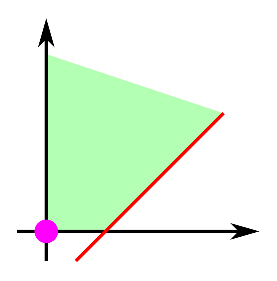
\includegraphics[width=4cm]{images/cone1.eps}}
\only<2>{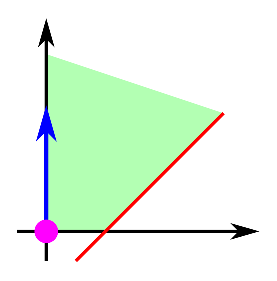
\includegraphics[width=4cm]{images/cone2.eps}}
\only<3>{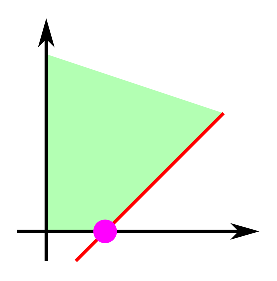
\includegraphics[width=4cm]{images/cone3.eps}}
\only<4>{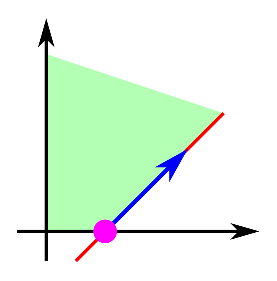
\includegraphics[width=4cm]{images/cone4.eps}}
\end{column}
\end{columns}

\end{frame}

\subsection{The convex hull problem}
\begin{frame}{The convex hull for bounded polyhedra}
In geometry, vertices and half-space are dual notions. The transformation is $a \leftrightarrow a.x \leq 1 $.
\begin{figure}
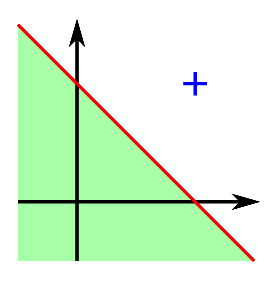
\includegraphics[scale=0.7]{images/dual.eps}

Duality between a vertex $(1,1)$ and an half-space $x+y \leq 1$
\end{figure}

\vspace*{-0.5cm}

\begin{theorem}
Let $P$ be a bounded polyhedron, if $0\in P$ then $P=P^{\Delta\Delta}$.
\end{theorem}

Starting from $P$, finding the vertices of $P^\Delta$ gives the convex hull of $P^{\Delta\Delta}$.
\end{frame}

\begin{frame}{An example of the convex hull algorithm}
\begin{itemize}
\visible<2->{\item Compute $P^\Delta$.}
\visible<3->{\item Enumerate the vertices.}
\visible<4->{\item Compute $P^{\Delta\Delta}$.}
\end{itemize}

\begin{figure}
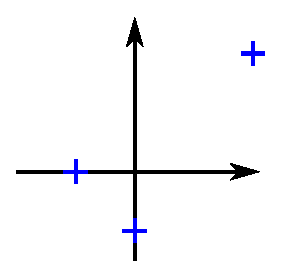
\includegraphics[scale=1]{images/dual11.eps}
\hspace*{0.5cm}
\only<2>{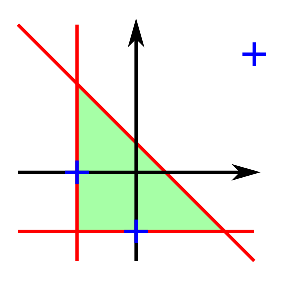
\includegraphics[scale=1]{images/dual2.eps}}
\only<3>{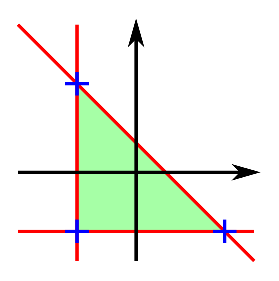
\includegraphics[scale=1]{images/dual3.eps}}
\only<4>{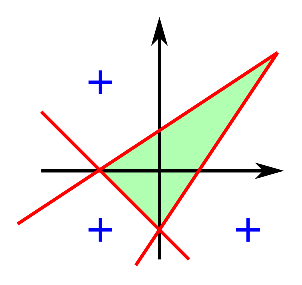
\includegraphics[scale=1]{images/dual4.eps}}
\only<5>{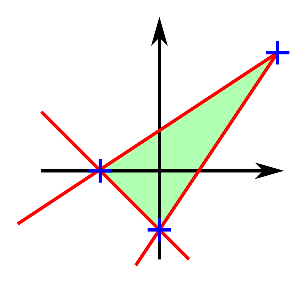
\includegraphics[scale=1]{images/dual5.eps}}

An example in two dimensions.
\end{figure}
\end{frame}

\begin{frame}{Finding the conic hull with the convex hull}
\begin{itemize}
\item consider the vectors as vertices and add the origin;
\item find the convex hull;
\item delete the hyperplanes not including the origin.
\end{itemize}
\begin{figure}
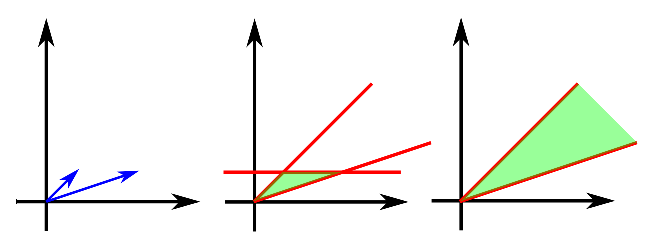
\includegraphics[scale=1]{images/conehull.eps}

An example in two dimensions.
\end{figure}
\end{frame}

\begin{frame}{The convex hull for polyhedron}
Any $V$-polyhedron $P=conv(V)+cone(C)$ can be written as the intersection of a cone and an hyperplane:

$P=Cone\left(
 \begin{pmatrix}
 0 \\
 C 
 \end{pmatrix},
 \begin{pmatrix}
 1 \\
 V 
 \end{pmatrix}\right) \cap \{(1,x)|x\in\mathbb{R}^d\}$
 
 %\vspace*{-0.7cm}
 
\begin{figure}

\includegraphics[scale=1.5]{images/projection.eps}

A $V$-polyhedron as an intersection.
\end{figure}
\end{frame}

\begin{frame}{Complexity result}
Theoretical complexity of Fukuda's algorithm: $nd(n+d)g$. $g\in \left[1;
\begin{pmatrix}
 d\\
 n 
 \end{pmatrix}\right]$

Cost of the algorithms:
\begin{itemize}
\item detect the linealty: cost of the simplex;
\item detect the cone: smaller than Fukuda's algorithm ($nd$ per vertex);
\item switch to the dual: $nd$.
\end{itemize} 

Faster than the current implementation, even in small dimension.

\end{frame}
